% https://tex.stackexchange.com/questions/188582/tikz-is-it-possible-to-draw-this-block-diagram
\documentclass[border=3pt]{standalone}
\usepackage{tikz}
\usetikzlibrary{positioning,fit,patterns}

\tikzset{
  pics/media/.style ={
    code = { %
      \node[text width=2cm,minimum height=2cm,#1] (back) {};
      \node[draw,anchor=center,fill=white] at ([yshift=5pt]back.center) {Media};
      \draw[dashed] (back.north west) rectangle (back.south east);
    }
  },
  pics/media/.default={pattern=north east lines},
  aes/.style={
    draw,
    fill=red!30
  },
  rsa/.style={
    draw,
    rounded corners,
    fill=blue!30
  },
  ar/.style={
    ->,
    >=latex,
    shorten >= 3pt,
    shorten <= 3pt,    
  },
  ar2/.style={
    ->,
    >=latex,
    line width=2pt,
    shorten >= 3pt,
    shorten <= 3pt,    
  }
}

\newcommand\mediaencryptedbox[3][1cm]{
\node[
  draw,
  thick,
  rounded corners,
  #2,
  text width=3.5cm,
  minimum height=4.5cm,
  anchor=north west,
  yshift=#1
  ]
  (#3)
  {};
\node[
  aes,
  anchor=north
  ]
  at (#3.north) 
  {AES key}; 
\pic at (#3.center) (sm3) {media};
\node[
  anchor=south
  ]
  (rsa)  
  at (sm3back.north) 
  {Encrypted with RSA};
\node[
  anchor=north
  ] 
  at (sm3back.south) 
  {Encrypted with AES};
\draw
  (#3.west|-rsa.south) -- (#3.east|-rsa.south);
}

\begin{document}

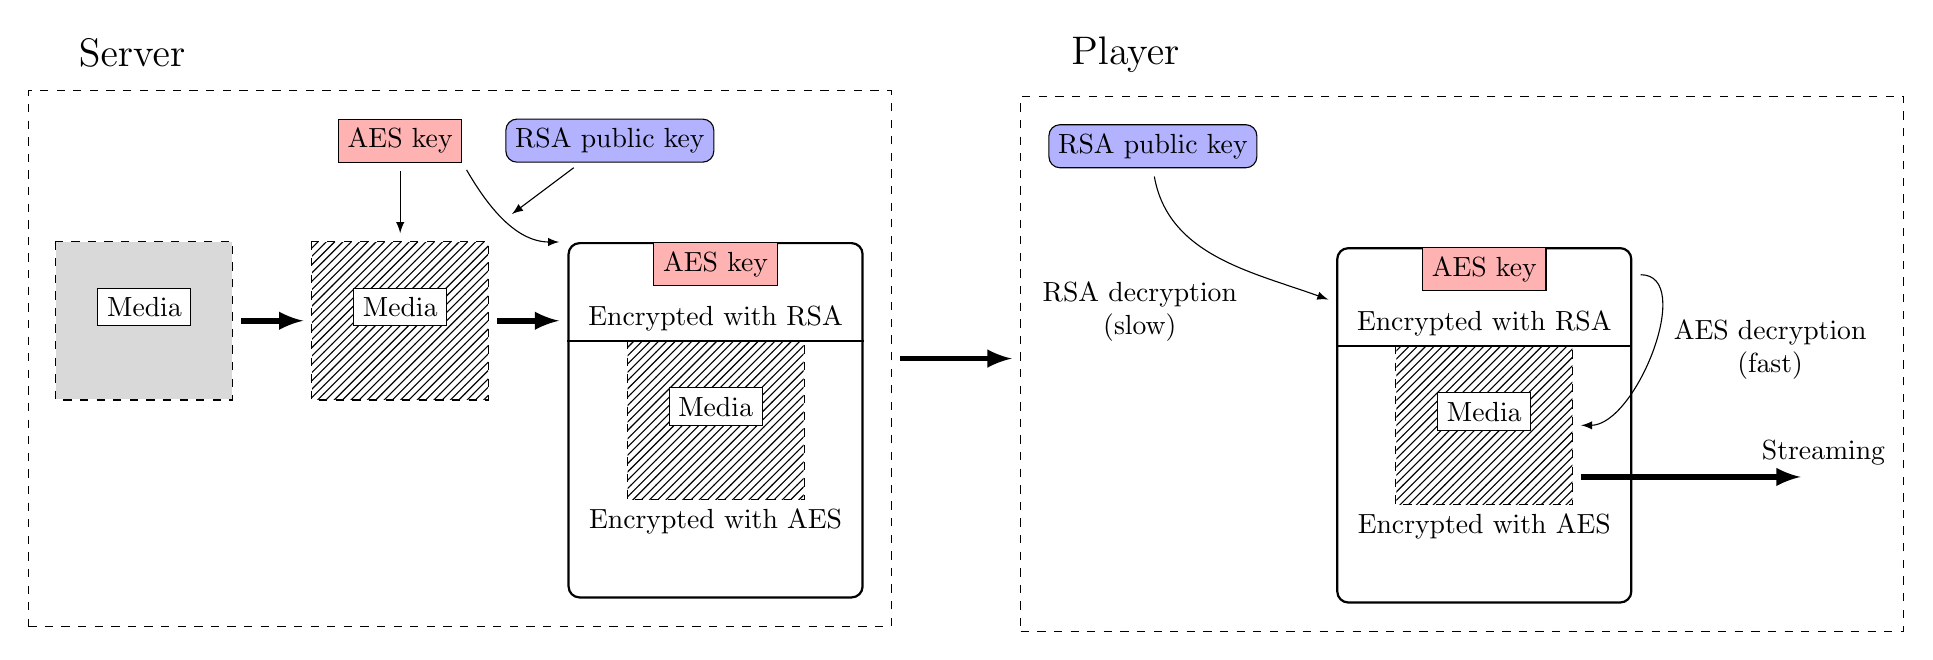
\begin{tikzpicture}

% The Server
\pic (sm1) {media={fill=gray!30}};
\pic[right=of sm1back] (sm2) {media};
\mediaencryptedbox{right=of sm2back}{box1}
\node[
  aes,
  anchor=north,
  above=of sm2back.north
  ]
  (aes1)
  {AES key};  
\draw[ar]
  (aes1) -- (sm2back.north) ;  
\draw[ar]
  (aes1.south east) to[out=-60,in=180] coordinate (aux1) (box1.north west) ;
\node[
  anchor=west,
  rsa
  ]
  at (aux1|-aes1)
  (rsa1)
  {RSA public key};    

\draw[ar]
  (rsa1) -- (aux1) ;  

\draw[ar2]
  (sm1back.east) -- (sm2back.west);
\draw[ar2]
  (sm2back.east) -- (box1.west|-sm2back.east);

\node[
  inner sep=10pt,
  draw,
  dashed,fit={(sm1back.north west) (box1.south east) (aes1)}
  ]
  (server) 
  {};
\node[
  anchor=south west,
  font=\Large
  ]
  at ([shift={(15pt,5pt)}]server.north west)
  {Server};      

% The Player
\mediaencryptedbox[2.2cm]{right=6cm of box1}{box2}
\node[
  anchor=north west,
  rsa,
  above left=of box2
  ]
  (rsa2)
  {RSA public key};    
\draw[ar]
  (rsa2.south) 
    to[out=-80,in=160]
    node[align=center,anchor=east,shift={(10pt,-20pt)}] {RSA decryption \\ (slow)} 
  ([yshift=-20pt]box2.north west);
\draw[ar]
  ([yshift=-10pt]box2.north east) 
    to[out=0,in=0]
    node[align=center,anchor=west,shift={(5pt,0pt)}] (AESd) {AES decryption \\ (fast)} 
  (sm3back.east);
\node[
  inner sep=10pt,
  draw,
  dashed,fit={(rsa2) (box2.south east) (AESd)}
  ]
  (player) 
  {};
\node[
  anchor=south west,
  font=\Large
  ]
  at ([shift={(15pt,5pt)}]player.north west)
  {Player};

\draw[ar2]
  (server.east) -- (player.west|-server.east);        
\draw[ar2]
  ([yshift=10pt]sm3back.south east) -- ++(3cm,0) node[near end,anchor=south west] {Streaming};
\end{tikzpicture}

\end{document}